%!TEX root = uist14.tex
\vfill
\section{Applications}
\label{sec:applications}

Head orientation targeting can enable a wide range of context-aware applications. We implement one particular demonstrative application: a universal smart appliance controller. Users select a smart device (e.g., light fixture, TV, or home appliance) with Glass --- upon confirming the selection, an device-specific UI is shown on the user's near-eye display, and they can control the application (without having to continually look at it) through their device touchpad.

We implemented a prototype of this remote controller for three physical devices: a lamp and fan that could be switched on or off and a smart TV control with playback, volume and navigation controls (see Figure~\ref{fig:smart-home}). We switched discrete appliances using relays, and implemented controls for a smart TV with a laptop connected to a 30\inch{} display. User interfaces for each were pre-defined in our application.

We set the devices up in a simulated living room environment and invited 14 users to step through a predefined set of tasks to control the appliances at a distance. 

%The huge benefit using head orientation is to solve two challenges that exist in most commercial list-based solutions -- {\em naming} and {\em scoping}. First, assigning clear names is non-trivial. Especially in shared spaces, the person trying to control the device might not be the one that named it - e.g., while an office building manager may know what ``Light 4 in area E'' corresponds to, an occupant may not. Second, without a method of scoping selection to automatically filter non-relevant devices, paging though long lists of names or navigating hierarchies becomes potentially more cumbersome than the physical action that the ``convenient'' software solution was meant to replace. Our head-orientation based interaction elegently solves these two problems.

%In order to control a smart appliance, the user performs a physical target selection (scan, refine and confirm) first and then the appliance-specific UI will be shown in the near-eye display. 

\begin{figure}[t]
\centering
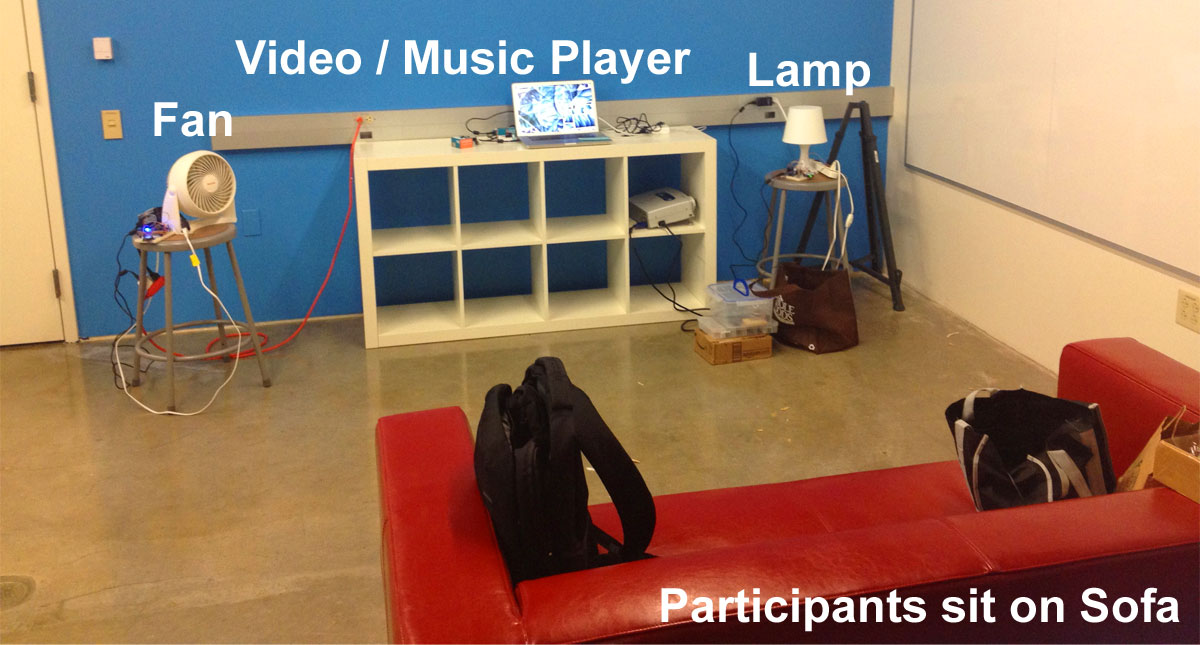
\includegraphics[width=0.95\columnwidth]{figures/smarthome-scenario.pdf}
\caption{In the smart home scenario, we have built three smart appliances for a user experience study. The interface supports both simple on/off appliances (lamp or fan) and multi-functional appliances (TV, for example).}
\label{fig:smart-home}
\end{figure}

%To assess the usability of such applications when the novel interaction scheme is added, we have built a few smart appliances (including a fan, a lamp and a TV, Figure~\ref{fig:smart-home}) and asked 14 participants to work through a concrete smart home scenario. The fan and lamp are relatively dumb and only support turning-on and turning-off. The smart TV provides control capability of switching the channels and adjust the volumn, as well as pause/play. From this study, we report some of the qualitative results to strength our motivation for the head-orientation interaction.

All participants successfully completed the list of tasks. They commented positively on the universal remote control functionality (e.g., \studyquote{I didn't have to search for different remote controllers for different appliances}) and stated it was easy to target and connect to appliances, in line with the findings of the previous study procedure. Participants saw potential benefits of the device for families; one user remarked that he could imagine people using the system \studyquote{while keeping an eye on their children at the same time}.

% \bjoern{1 is problematic - because it sounds like that the head worn device is in the end not worth it and you should just use your phone, even if it takes longer. I'm not sure we can confidently say something about museums or body shops - this sounds speculative. Needs section needs to be rephrased., e.g. as in: Our solution succeeds at X because of Y. This suggests that future applications in domains like Z could be especially promising.}

\changes{Though our solution successfully solves the problem of {\em target selection}, we have not fully addressed the issue of controlling smart devices. One user reported that \studyquote{for more complex appliances (TV), interaction was more difficult}. A separate work on interaction techniques for head-worn computing devices is needed to address these issues, while we keep our focus on target selection. When the device is more complicated, it is possible that a better solution may be a hybrid -- to select the appliance with HOBS and control it with a phone.} \claire{ Is it possible to say that the number of complicated devices that you want to remote control is limited almost exclusively to the tv? I can't think of too many of these devices and our system works very well with more simple devices, which seem to be more common.} \sean{ I wouldn't state that. We could be challenged if the reviewers bring up smart fridge, microwave, etc.}

%% I feel like we should mention a bit about the interaction complexity. But that's a bit out of the scope of this paper.
%% Participants rated the ease of control of particular appliances differently. Ease of use ratings were higher for the lamp and fan which had simple, discrete on/off actions, and lower for the more complex movie player (see Figure~\ref{fig:smarthome-likert}). Multiple participants remarked that the difficulty was based on the affordances of Glass: \studyquote{Most of the difficulty I had with Glass came from having to navigate the interface on the tiny screen with the touch pad}. The screen size and (largely) 1D input put a limit on the complexity of interfaces that can be presented. As one participant remarked: \studyquote{[The media player] does not seem to be more efficient than a tablet device.} The difficulty can also partly be ascribed to our interaction design, which required one finger swipes to switch between parameters and two finger gestures for adjusting parameters --- it was hard for users to exert fine control over two-finger swipes. In addition, users did not always remember these mappings as they are not yet part of a standard gesture vocabulary.


%%% Local Variables: 
%%% mode: latex
%%% TeX-master: "uist14"
%%% End: 
